\documentclass[1p]{elsarticle_modified}
%\bibliographystyle{elsarticle-num}

%\usepackage[colorlinks]{hyperref}
%\usepackage{abbrmath_seonhwa} %\Abb, \Ascr, \Acal ,\Abf, \Afrak
\usepackage{amsfonts}
\usepackage{amssymb}
\usepackage{amsmath}
\usepackage{amsthm}
\usepackage{scalefnt}
\usepackage{amsbsy}
\usepackage{kotex}
\usepackage{caption}
\usepackage{subfig}
\usepackage{color}
\usepackage{graphicx}
\usepackage{xcolor} %% white, black, red, green, blue, cyan, magenta, yellow
\usepackage{float}
\usepackage{setspace}
\usepackage{hyperref}

\usepackage{tikz}
\usetikzlibrary{arrows}

\usepackage{multirow}
\usepackage{array} % fixed length table
\usepackage{hhline}

%%%%%%%%%%%%%%%%%%%%%
\makeatletter
\renewcommand*\env@matrix[1][\arraystretch]{%
	\edef\arraystretch{#1}%
	\hskip -\arraycolsep
	\let\@ifnextchar\new@ifnextchar
	\array{*\c@MaxMatrixCols c}}
\makeatother %https://tex.stackexchange.com/questions/14071/how-can-i-increase-the-line-spacing-in-a-matrix
%%%%%%%%%%%%%%%

\usepackage[normalem]{ulem}

\newcommand{\msout}[1]{\ifmmode\text{\sout{\ensuremath{#1}}}\else\sout{#1}\fi}
%SOURCE: \msout is \stkout macro in https://tex.stackexchange.com/questions/20609/strikeout-in-math-mode

\newcommand{\cancel}[1]{
	\ifmmode
	{\color{red}\msout{#1}}
	\else
	{\color{red}\sout{#1}}
	\fi
}

\newcommand{\add}[1]{
	{\color{blue}\uwave{#1}}
}

\newcommand{\replace}[2]{
	\ifmmode
	{\color{red}\msout{#1}}{\color{blue}\uwave{#2}}
	\else
	{\color{red}\sout{#1}}{\color{blue}\uwave{#2}}
	\fi
}

\newcommand{\Sol}{\mathcal{S}} %segment
\newcommand{\D}{D} %diagram
\newcommand{\A}{\mathcal{A}} %arc


%%%%%%%%%%%%%%%%%%%%%%%%%%%%%5 test

\def\sl{\operatorname{\textup{SL}}(2,\Cbb)}
\def\psl{\operatorname{\textup{PSL}}(2,\Cbb)}
\def\quan{\mkern 1mu \triangleright \mkern 1mu}

\theoremstyle{definition}
\newtheorem{thm}{Theorem}[section]
\newtheorem{prop}[thm]{Proposition}
\newtheorem{lem}[thm]{Lemma}
\newtheorem{ques}[thm]{Question}
\newtheorem{cor}[thm]{Corollary}
\newtheorem{defn}[thm]{Definition}
\newtheorem{exam}[thm]{Example}
\newtheorem{rmk}[thm]{Remark}
\newtheorem{alg}[thm]{Algorithm}

\newcommand{\I}{\sqrt{-1}}
\begin{document}

%\begin{frontmatter}
%
%\title{Boundary parabolic representations of knots up to 8 crossings}
%
%%% Group authors per affiliation:
%\author{Yunhi Cho} 
%\address{Department of Mathematics, University of Seoul, Seoul, Korea}
%\ead{yhcho@uos.ac.kr}
%
%
%\author{Seonhwa Kim} %\fnref{s_kim}}
%\address{Center for Geometry and Physics, Institute for Basic Science, Pohang, 37673, Korea}
%\ead{ryeona17@ibs.re.kr}
%
%\author{Hyuk Kim}
%\address{Department of Mathematical Sciences, Seoul National University, Seoul 08826, Korea}
%\ead{hyukkim@snu.ac.kr}
%
%\author{Seokbeom Yoon}
%\address{Department of Mathematical Sciences, Seoul National University, Seoul, 08826,  Korea}
%\ead{sbyoon15@snu.ac.kr}
%
%\begin{abstract}
%We find all boundary parabolic representation of knots up to 8 crossings.
%
%\end{abstract}
%\begin{keyword}
%    \MSC[2010] 57M25 
%\end{keyword}
%
%\end{frontmatter}

%\linenumbers
%\tableofcontents
%
\newcommand\colored[1]{\textcolor{white}{\rule[-0.35ex]{0.8em}{1.4ex}}\kern-0.8em\color{red} #1}%
%\newcommand\colored[1]{\textcolor{white}{ #1}\kern-2.17ex	\textcolor{white}{ #1}\kern-1.81ex	\textcolor{white}{ #1}\kern-2.15ex\color{red}#1	}

{\Large $\underline{11a_{248}~(K11a_{248})}$}

\setlength{\tabcolsep}{10pt}
\renewcommand{\arraystretch}{1.6}
\vspace{1cm}\begin{tabular}{m{100pt}>{\centering\arraybackslash}m{274pt}}
\multirow{5}{120pt}{
	\centering
	\includegraphics[width=112pt]{../../../GIT/diagram.site/Diagrams/png/497_11a_248.png}\\
\ \ \ A knot diagram\footnotemark}&
\allowdisplaybreaks
\textbf{Linearized knot diagam} \\
\cline{2-2}
 &
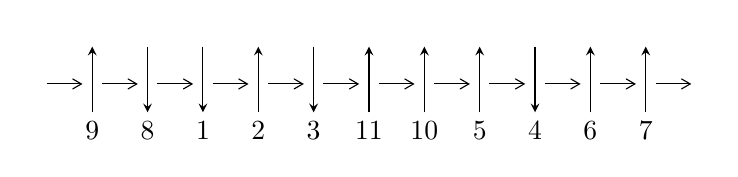
\begin{tikzpicture}[x=20pt, y=17pt]
	% nodes
	\node (C0) at (0, 0) {};
	\node (C1) at (1, 0) {};
	\node (C1U) at (1, +1) {};
	\node (C1D) at (1, -1) {9};

	\node (C2) at (2, 0) {};
	\node (C2U) at (2, +1) {};
	\node (C2D) at (2, -1) {8};

	\node (C3) at (3, 0) {};
	\node (C3U) at (3, +1) {};
	\node (C3D) at (3, -1) {1};

	\node (C4) at (4, 0) {};
	\node (C4U) at (4, +1) {};
	\node (C4D) at (4, -1) {2};

	\node (C5) at (5, 0) {};
	\node (C5U) at (5, +1) {};
	\node (C5D) at (5, -1) {3};

	\node (C6) at (6, 0) {};
	\node (C6U) at (6, +1) {};
	\node (C6D) at (6, -1) {11};

	\node (C7) at (7, 0) {};
	\node (C7U) at (7, +1) {};
	\node (C7D) at (7, -1) {10};

	\node (C8) at (8, 0) {};
	\node (C8U) at (8, +1) {};
	\node (C8D) at (8, -1) {5};

	\node (C9) at (9, 0) {};
	\node (C9U) at (9, +1) {};
	\node (C9D) at (9, -1) {4};

	\node (C10) at (10, 0) {};
	\node (C10U) at (10, +1) {};
	\node (C10D) at (10, -1) {6};

	\node (C11) at (11, 0) {};
	\node (C11U) at (11, +1) {};
	\node (C11D) at (11, -1) {7};
	\node (C12) at (12, 0) {};

	% arrows
	\draw[->,>={angle 60}]
	(C0) edge (C1) (C1) edge (C2) (C2) edge (C3) (C3) edge (C4) (C4) edge (C5) (C5) edge (C6) (C6) edge (C7) (C7) edge (C8) (C8) edge (C9) (C9) edge (C10) (C10) edge (C11) (C11) edge (C12) ;	\draw[->,>=stealth]
	(C1D) edge (C1U) (C2U) edge (C2D) (C3U) edge (C3D) (C4D) edge (C4U) (C5U) edge (C5D) (C6D) edge (C6U) (C7D) edge (C7U) (C8D) edge (C8U) (C9U) edge (C9D) (C10D) edge (C10U) (C11D) edge (C11U) ;
	\end{tikzpicture} \\
\hhline{~~} \\& 
\textbf{Solving Sequence} \\ \cline{2-2} 
 &
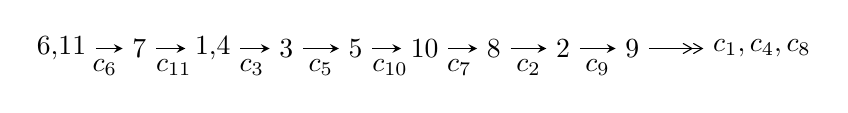
\begin{tikzpicture}[x=25pt, y=7pt]
	% node
	\node (A0) at (-1/8, 0) {6,11};
	\node (A1) at (1, 0) {7};
	\node (A2) at (33/16, 0) {1,4};
	\node (A3) at (25/8, 0) {3};
	\node (A4) at (33/8, 0) {5};
	\node (A5) at (41/8, 0) {10};
	\node (A6) at (49/8, 0) {8};
	\node (A7) at (57/8, 0) {2};
	\node (A8) at (65/8, 0) {9};
	\node (C1) at (1/2, -1) {$c_{6}$};
	\node (C2) at (3/2, -1) {$c_{11}$};
	\node (C3) at (21/8, -1) {$c_{3}$};
	\node (C4) at (29/8, -1) {$c_{5}$};
	\node (C5) at (37/8, -1) {$c_{10}$};
	\node (C6) at (45/8, -1) {$c_{7}$};
	\node (C7) at (53/8, -1) {$c_{2}$};
	\node (C8) at (61/8, -1) {$c_{9}$};
	\node (A9) at (10, 0) {$c_{1},c_{4},c_{8}$};

	% edge
	\draw[->,>=stealth]	
	(A0) edge (A1) (A1) edge (A2) (A2) edge (A3) (A3) edge (A4) (A4) edge (A5) (A5) edge (A6) (A6) edge (A7) (A7) edge (A8) ;
	\draw[->>,>={angle 60}]	
	(A8) edge (A9);
\end{tikzpicture} \\ 

\end{tabular} \\

\footnotetext{
The image of knot diagram is generated by the software ``\textbf{Draw programme}" developed by Andrew Bartholomew(\url{http://www.layer8.co.uk/maths/draw/index.htm\#Running-draw}), where we modified some parts for our purpose(\url{https://github.com/CATsTAILs/LinksPainter}).
}\phantom \\ \newline 
\centering \textbf{Ideals for irreducible components\footnotemark of $X_{\text{par}}$} 
 
\begin{align*}
I^u_{1}&=\langle 
-7806 u^{39}-28939 u^{38}+\cdots+1091 b+30599,\;20501 u^{39}+69845 u^{38}+\cdots+4364 a-128043,\\
\phantom{I^u_{1}}&\phantom{= \langle  }u^{40}+5 u^{39}+\cdots+9 u-4\rangle \\
I^u_{2}&=\langle 
u^{26} a+u^{26}+\cdots+b- u,\;-4 u^{26} a+4 u^{26}+\cdots- a+5,\;u^{27}-2 u^{26}+\cdots-4 u^2-1\rangle \\
I^u_{3}&=\langle 
- u^{11}+6 u^9+u^8-12 u^7-5 u^6+8 u^5+7 u^4+2 u^3-2 u^2+b-3 u,\\
\phantom{I^u_{3}}&\phantom{= \langle  }u^{12}-6 u^{10}- u^9+13 u^8+4 u^7-11 u^6-6 u^5+u^4+4 u^3+3 u^2+a-2 u-2,\\
\phantom{I^u_{3}}&\phantom{= \langle  }u^{13}-2 u^{12}-5 u^{11}+10 u^{10}+10 u^9-17 u^8-11 u^7+8 u^6+7 u^5+7 u^4- u^3-7 u^2-1\rangle \\
I^u_{4}&=\langle 
b+1,\;a^2-3 a+3,\;u+1\rangle \\
\\
\end{align*}
\raggedright * 4 irreducible components of $\dim_{\mathbb{C}}=0$, with total 109 representations.\\
\footnotetext{All coefficients of polynomials are rational numbers. But the coefficients are sometimes approximated in decimal forms when there is not enough margin.}
\newpage
\renewcommand{\arraystretch}{1}
\centering \section*{I. $I^u_{1}= \langle -7806 u^{39}-28939 u^{38}+\cdots+1091 b+30599,\;20501 u^{39}+69845 u^{38}+\cdots+4364 a-128043,\;u^{40}+5 u^{39}+\cdots+9 u-4 \rangle$}
\flushleft \textbf{(i) Arc colorings}\\
\begin{tabular}{m{7pt} m{180pt} m{7pt} m{180pt} }
\flushright $a_{6}=$&$\begin{pmatrix}1\\0\end{pmatrix}$ \\
\flushright $a_{11}=$&$\begin{pmatrix}0\\u\end{pmatrix}$ \\
\flushright $a_{7}=$&$\begin{pmatrix}1\\- u^2\end{pmatrix}$ \\
\flushright $a_{1}=$&$\begin{pmatrix}u\\- u^3+u\end{pmatrix}$ \\
\flushright $a_{4}=$&$\begin{pmatrix}-4.69775 u^{39}-16.0048 u^{38}+\cdots-70.7569 u+29.3407\\7.15490 u^{39}+26.5252 u^{38}+\cdots+78.3217 u-28.0467\end{pmatrix}$ \\
\flushright $a_{3}=$&$\begin{pmatrix}12.9365 u^{39}+44.7789 u^{38}+\cdots+77.7912 u-24.2945\\-13.4088 u^{39}-49.4097 u^{38}+\cdots-90.1567 u+27.8689\end{pmatrix}$ \\
\flushright $a_{5}=$&$\begin{pmatrix}-7.68492 u^{39}-28.0323 u^{38}+\cdots-26.6533 u+1.57356\\11.5527 u^{39}+43.6728 u^{38}+\cdots+54.5325 u-10.8295\end{pmatrix}$ \\
\flushright $a_{10}=$&$\begin{pmatrix}- u\\u\end{pmatrix}$ \\
\flushright $a_{8}=$&$\begin{pmatrix}- u^4+u^2+1\\u^4-2 u^2\end{pmatrix}$ \\
\flushright $a_{2}=$&$\begin{pmatrix}7.93103 u^{39}+26.6478 u^{38}+\cdots+51.3183 u-18.2514\\-11.2988 u^{39}-41.7883 u^{38}+\cdots-83.6975 u+27.0073\end{pmatrix}$ \\
\flushright $a_{9}=$&$\begin{pmatrix}1.73854 u^{39}+0.0602658 u^{38}+\cdots+26.7647 u-19.7436\\-1.46379 u^{39}-2.72044 u^{38}+\cdots-15.8863 u+10.2997\end{pmatrix}$\\ \flushright $a_{9}=$&$\begin{pmatrix}1.73854 u^{39}+0.0602658 u^{38}+\cdots+26.7647 u-19.7436\\-1.46379 u^{39}-2.72044 u^{38}+\cdots-15.8863 u+10.2997\end{pmatrix}$\\&\end{tabular}
\flushleft \textbf{(ii) Obstruction class $= -1$}\\~\\
\flushleft \textbf{(iii) Cusp Shapes $= -\frac{10012}{1091} u^{39}-\frac{44785}{1091} u^{38}+\cdots+\frac{78319}{1091} u-\frac{64130}{1091}$}\\~\\
\newpage\renewcommand{\arraystretch}{1}
\flushleft \textbf{(iv) u-Polynomials at the component}\newline \\
\begin{tabular}{m{50pt}|m{274pt}}
Crossings & \hspace{64pt}u-Polynomials at each crossing \\
\hline $$\begin{aligned}c_{1},c_{8}\end{aligned}$$&$\begin{aligned}
&u^{40}- u^{39}+\cdots+2 u-1
\end{aligned}$\\
\hline $$\begin{aligned}c_{2},c_{9}\end{aligned}$$&$\begin{aligned}
&u^{40}+2 u^{38}+\cdots- u-1
\end{aligned}$\\
\hline $$\begin{aligned}c_{3},c_{5}\end{aligned}$$&$\begin{aligned}
&u^{40}+6 u^{39}+\cdots-23 u+1
\end{aligned}$\\
\hline $$\begin{aligned}c_{4}\end{aligned}$$&$\begin{aligned}
&u^{40}+22 u^{39}+\cdots+9 u+2
\end{aligned}$\\
\hline $$\begin{aligned}c_{6},c_{10},c_{11}\end{aligned}$$&$\begin{aligned}
&u^{40}-5 u^{39}+\cdots-9 u-4
\end{aligned}$\\
\hline $$\begin{aligned}c_{7}\end{aligned}$$&$\begin{aligned}
&u^{40}+15 u^{39}+\cdots+89 u+4
\end{aligned}$\\
\hline
\end{tabular}\\~\\
\newpage\renewcommand{\arraystretch}{1}
\flushleft \textbf{(v) Riley Polynomials at the component}\newline \\
\begin{tabular}{m{50pt}|m{274pt}}
Crossings & \hspace{64pt}Riley Polynomials at each crossing \\
\hline $$\begin{aligned}c_{1},c_{8}\end{aligned}$$&$\begin{aligned}
&y^{40}+17 y^{39}+\cdots+44 y+1
\end{aligned}$\\
\hline $$\begin{aligned}c_{2},c_{9}\end{aligned}$$&$\begin{aligned}
&y^{40}+4 y^{39}+\cdots-23 y+1
\end{aligned}$\\
\hline $$\begin{aligned}c_{3},c_{5}\end{aligned}$$&$\begin{aligned}
&y^{40}-24 y^{39}+\cdots-199 y+1
\end{aligned}$\\
\hline $$\begin{aligned}c_{4}\end{aligned}$$&$\begin{aligned}
&y^{40}+28 y^{38}+\cdots-5 y+4
\end{aligned}$\\
\hline $$\begin{aligned}c_{6},c_{10},c_{11}\end{aligned}$$&$\begin{aligned}
&y^{40}-37 y^{39}+\cdots-9 y+16
\end{aligned}$\\
\hline $$\begin{aligned}c_{7}\end{aligned}$$&$\begin{aligned}
&y^{40}- y^{39}+\cdots-937 y+16
\end{aligned}$\\
\hline
\end{tabular}\\~\\
\newpage\flushleft \textbf{(vi) Complex Volumes and Cusp Shapes}
$$\begin{array}{c|c|c}  
\text{Solutions to }I^u_{1}& \I (\text{vol} + \sqrt{-1}CS) & \text{Cusp shape}\\
 \hline 
\begin{aligned}
u &= \phantom{-}0.833239 + 0.478940 I \\
a &= \phantom{-}1.36899 + 1.05581 I \\
b &= \phantom{-}0.113249 - 0.613771 I\end{aligned}
 & -0.67356 - 9.11808 I & \phantom{-}3.09330 + 5.04292 I \\ \hline\begin{aligned}
u &= \phantom{-}0.833239 - 0.478940 I \\
a &= \phantom{-}1.36899 - 1.05581 I \\
b &= \phantom{-}0.113249 + 0.613771 I\end{aligned}
 & -0.67356 + 9.11808 I & \phantom{-}3.09330 - 5.04292 I \\ \hline\begin{aligned}
u &= \phantom{-}0.944818 + 0.044872 I \\
a &= -1.88518 - 0.83264 I \\
b &= \phantom{-}1.092540 + 0.590515 I\end{aligned}
 & -1.64126 - 1.68382 I & -2.62360 + 4.24820 I \\ \hline\begin{aligned}
u &= \phantom{-}0.944818 - 0.044872 I \\
a &= -1.88518 + 0.83264 I \\
b &= \phantom{-}1.092540 - 0.590515 I\end{aligned}
 & -1.64126 + 1.68382 I & -2.62360 - 4.24820 I \\ \hline\begin{aligned}
u &= \phantom{-}1.045020 + 0.426092 I \\
a &= \phantom{-}1.40350 - 0.24037 I \\
b &= -0.777991 - 0.700678 I\end{aligned}
 & -1.51874 + 7.98713 I & \phantom{-}1.00079 - 8.43785 I \\ \hline\begin{aligned}
u &= \phantom{-}1.045020 - 0.426092 I \\
a &= \phantom{-}1.40350 + 0.24037 I \\
b &= -0.777991 + 0.700678 I\end{aligned}
 & -1.51874 - 7.98713 I & \phantom{-}1.00079 + 8.43785 I \\ \hline\begin{aligned}
u &= \phantom{-}0.127215 + 0.839082 I \\
a &= -0.212294 + 0.072049 I \\
b &= -0.507546 + 1.079890 I\end{aligned}
 & -4.35513 - 3.45950 I & -3.88332 + 4.09172 I \\ \hline\begin{aligned}
u &= \phantom{-}0.127215 - 0.839082 I \\
a &= -0.212294 - 0.072049 I \\
b &= -0.507546 - 1.079890 I\end{aligned}
 & -4.35513 + 3.45950 I & -3.88332 - 4.09172 I \\ \hline\begin{aligned}
u &= \phantom{-}0.277504 + 0.801125 I \\
a &= \phantom{-}0.171151 - 0.043121 I \\
b &= \phantom{-}0.77473 + 1.69376 I\end{aligned}
 & -2.45998 + 13.64270 I & \phantom{-}1.03420 - 9.07195 I \\ \hline\begin{aligned}
u &= \phantom{-}0.277504 - 0.801125 I \\
a &= \phantom{-}0.171151 + 0.043121 I \\
b &= \phantom{-}0.77473 - 1.69376 I\end{aligned}
 & -2.45998 - 13.64270 I & \phantom{-}1.03420 + 9.07195 I\\
 \hline 
 \end{array}$$\newpage$$\begin{array}{c|c|c}  
\text{Solutions to }I^u_{1}& \I (\text{vol} + \sqrt{-1}CS) & \text{Cusp shape}\\
 \hline 
\begin{aligned}
u &= -0.777292\phantom{ +0.000000I} \\
a &= -0.568128\phantom{ +0.000000I} \\
b &= -0.113354\phantom{ +0.000000I}\end{aligned}
 & \phantom{-}1.36099\phantom{ +0.000000I} & \phantom{-}8.46400\phantom{ +0.000000I} \\ \hline\begin{aligned}
u &= \phantom{-}0.225491 + 0.702834 I \\
a &= \phantom{-}0.212358 + 0.335622 I \\
b &= -0.39127 - 1.71232 I\end{aligned}
 & -3.63204 + 5.12135 I & -5.87713 - 8.64312 I \\ \hline\begin{aligned}
u &= \phantom{-}0.225491 - 0.702834 I \\
a &= \phantom{-}0.212358 - 0.335622 I \\
b &= -0.39127 + 1.71232 I\end{aligned}
 & -3.63204 - 5.12135 I & -5.87713 + 8.64312 I \\ \hline\begin{aligned}
u &= \phantom{-}0.290696 + 0.655817 I \\
a &= -0.279795 + 0.357972 I \\
b &= \phantom{-}0.417996 - 0.903025 I\end{aligned}
 & -3.25229 + 1.41438 I & -4.70580 - 2.22096 I \\ \hline\begin{aligned}
u &= \phantom{-}0.290696 - 0.655817 I \\
a &= -0.279795 - 0.357972 I \\
b &= \phantom{-}0.417996 + 0.903025 I\end{aligned}
 & -3.25229 - 1.41438 I & -4.70580 + 2.22096 I \\ \hline\begin{aligned}
u &= -1.283570 + 0.210194 I \\
a &= \phantom{-}0.89404 - 1.55425 I \\
b &= -0.229292 + 0.859047 I\end{aligned}
 & \phantom{-}1.12425 - 2.76728 I & \phantom{-0.000000 -}0. + 3.97586 I \\ \hline\begin{aligned}
u &= -1.283570 - 0.210194 I \\
a &= \phantom{-}0.89404 + 1.55425 I \\
b &= -0.229292 - 0.859047 I\end{aligned}
 & \phantom{-}1.12425 + 2.76728 I & \phantom{-0.000000 } 0. - 3.97586 I \\ \hline\begin{aligned}
u &= \phantom{-}1.317130 + 0.218392 I \\
a &= -2.22707 - 0.75204 I \\
b &= \phantom{-}2.17192 + 1.88185 I\end{aligned}
 & \phantom{-}1.43716 + 2.94730 I & \phantom{-0.000000 } 0 \\ \hline\begin{aligned}
u &= \phantom{-}1.317130 - 0.218392 I \\
a &= -2.22707 + 0.75204 I \\
b &= \phantom{-}2.17192 - 1.88185 I\end{aligned}
 & \phantom{-}1.43716 - 2.94730 I & \phantom{-0.000000 } 0 \\ \hline\begin{aligned}
u &= \phantom{-}0.646576 + 0.028959 I \\
a &= -1.71193 - 0.86713 I \\
b &= \phantom{-}0.662046 + 0.361055 I\end{aligned}
 & -1.67832 - 1.69625 I & -1.45396 + 4.31564 I\\
 \hline 
 \end{array}$$\newpage$$\begin{array}{c|c|c}  
\text{Solutions to }I^u_{1}& \I (\text{vol} + \sqrt{-1}CS) & \text{Cusp shape}\\
 \hline 
\begin{aligned}
u &= \phantom{-}0.646576 - 0.028959 I \\
a &= -1.71193 + 0.86713 I \\
b &= \phantom{-}0.662046 - 0.361055 I\end{aligned}
 & -1.67832 + 1.69625 I & -1.45396 - 4.31564 I \\ \hline\begin{aligned}
u &= -1.307710 + 0.361702 I \\
a &= -0.730497 + 0.872523 I \\
b &= -0.038517 - 0.940647 I\end{aligned}
 & \phantom{-}0.125718 - 0.859000 I & \phantom{-0.000000 } 0 \\ \hline\begin{aligned}
u &= -1.307710 - 0.361702 I \\
a &= -0.730497 - 0.872523 I \\
b &= -0.038517 + 0.940647 I\end{aligned}
 & \phantom{-}0.125718 + 0.859000 I & \phantom{-0.000000 } 0 \\ \hline\begin{aligned}
u &= -1.374750 + 0.100729 I \\
a &= -0.937295 + 0.058184 I \\
b &= \phantom{-}0.401012 + 0.417839 I\end{aligned}
 & \phantom{-}4.00380 + 0.89695 I & \phantom{-0.000000 } 0 \\ \hline\begin{aligned}
u &= -1.374750 - 0.100729 I \\
a &= -0.937295 - 0.058184 I \\
b &= \phantom{-}0.401012 - 0.417839 I\end{aligned}
 & \phantom{-}4.00380 - 0.89695 I & \phantom{-0.000000 } 0 \\ \hline\begin{aligned}
u &= \phantom{-}1.395900 + 0.204775 I \\
a &= \phantom{-}1.022420 + 0.746778 I \\
b &= -0.98876 - 1.47035 I\end{aligned}
 & \phantom{-}5.90256 + 4.07376 I & \phantom{-0.000000 } 0 \\ \hline\begin{aligned}
u &= \phantom{-}1.395900 - 0.204775 I \\
a &= \phantom{-}1.022420 - 0.746778 I \\
b &= -0.98876 + 1.47035 I\end{aligned}
 & \phantom{-}5.90256 - 4.07376 I & \phantom{-0.000000 } 0 \\ \hline\begin{aligned}
u &= -1.38885 + 0.28086 I \\
a &= \phantom{-}2.23443 - 1.30007 I \\
b &= -1.61945 + 1.79021 I\end{aligned}
 & \phantom{-}1.50108 - 8.69698 I & \phantom{-0.000000 } 0 \\ \hline\begin{aligned}
u &= -1.38885 - 0.28086 I \\
a &= \phantom{-}2.23443 + 1.30007 I \\
b &= -1.61945 - 1.79021 I\end{aligned}
 & \phantom{-}1.50108 + 8.69698 I & \phantom{-0.000000 } 0 \\ \hline\begin{aligned}
u &= -0.024475 + 0.578228 I \\
a &= \phantom{-}1.202030 + 0.432697 I \\
b &= \phantom{-}0.84787 - 1.24338 I\end{aligned}
 & -2.81557 - 0.07740 I & -5.03252 - 0.22412 I\\
 \hline 
 \end{array}$$\newpage$$\begin{array}{c|c|c}  
\text{Solutions to }I^u_{1}& \I (\text{vol} + \sqrt{-1}CS) & \text{Cusp shape}\\
 \hline 
\begin{aligned}
u &= -0.024475 - 0.578228 I \\
a &= \phantom{-}1.202030 - 0.432697 I \\
b &= \phantom{-}0.84787 + 1.24338 I\end{aligned}
 & -2.81557 + 0.07740 I & -5.03252 + 0.22412 I \\ \hline\begin{aligned}
u &= -0.293128 + 0.498415 I \\
a &= -0.724756 + 0.441160 I \\
b &= -0.324784 + 0.529368 I\end{aligned}
 & \phantom{-}0.54657 - 1.42879 I & \phantom{-}5.31935 + 4.51277 I \\ \hline\begin{aligned}
u &= -0.293128 - 0.498415 I \\
a &= -0.724756 - 0.441160 I \\
b &= -0.324784 - 0.529368 I\end{aligned}
 & \phantom{-}0.54657 + 1.42879 I & \phantom{-}5.31935 - 4.51277 I \\ \hline\begin{aligned}
u &= -1.43383 + 0.26362 I \\
a &= \phantom{-}0.738341 - 1.202280 I \\
b &= -0.54490 + 1.45255 I\end{aligned}
 & \phantom{-}2.31251 - 4.79347 I & \phantom{-0.000000 } 0 \\ \hline\begin{aligned}
u &= -1.43383 - 0.26362 I \\
a &= \phantom{-}0.738341 + 1.202280 I \\
b &= -0.54490 - 1.45255 I\end{aligned}
 & \phantom{-}2.31251 + 4.79347 I & \phantom{-0.000000 } 0 \\ \hline\begin{aligned}
u &= -1.42214 + 0.32372 I \\
a &= -2.22593 + 1.15650 I \\
b &= \phantom{-}1.72849 - 2.18761 I\end{aligned}
 & \phantom{-}2.9545 - 17.7145 I & \phantom{-0.000000 } 0 \\ \hline\begin{aligned}
u &= -1.42214 - 0.32372 I \\
a &= -2.22593 - 1.15650 I \\
b &= \phantom{-}1.72849 + 2.18761 I\end{aligned}
 & \phantom{-}2.9545 + 17.7145 I & \phantom{-0.000000 } 0 \\ \hline\begin{aligned}
u &= -1.51106 + 0.03418 I \\
a &= -0.041421 + 0.318529 I \\
b &= \phantom{-}0.551162 - 0.994771 I\end{aligned}
 & \phantom{-}7.13383 + 7.90887 I & \phantom{-0.000000 } 0 \\ \hline\begin{aligned}
u &= -1.51106 - 0.03418 I \\
a &= -0.041421 - 0.318529 I \\
b &= \phantom{-}0.551162 + 0.994771 I\end{aligned}
 & \phantom{-}7.13383 - 7.90887 I & \phantom{-0.000000 } 0 \\ \hline\begin{aligned}
u &= \phantom{-}1.64915\phantom{ +0.000000I} \\
a &= \phantom{-}0.275951\phantom{ +0.000000I} \\
b &= -0.563647\phantom{ +0.000000I}\end{aligned}
 & \phantom{-}9.99305\phantom{ +0.000000I} & \phantom{-0.000000 } 0\\
 \hline 
 \end{array}$$\newpage\newpage\renewcommand{\arraystretch}{1}
\centering \section*{II. $I^u_{2}= \langle u^{26} a+u^{26}+\cdots+b- u,\;-4 u^{26} a+4 u^{26}+\cdots- a+5,\;u^{27}-2 u^{26}+\cdots-4 u^2-1 \rangle$}
\flushleft \textbf{(i) Arc colorings}\\
\begin{tabular}{m{7pt} m{180pt} m{7pt} m{180pt} }
\flushright $a_{6}=$&$\begin{pmatrix}1\\0\end{pmatrix}$ \\
\flushright $a_{11}=$&$\begin{pmatrix}0\\u\end{pmatrix}$ \\
\flushright $a_{7}=$&$\begin{pmatrix}1\\- u^2\end{pmatrix}$ \\
\flushright $a_{1}=$&$\begin{pmatrix}u\\- u^3+u\end{pmatrix}$ \\
\flushright $a_{4}=$&$\begin{pmatrix}a\\- u^{26} a- u^{26}+\cdots+a u+u\end{pmatrix}$ \\
\flushright $a_{3}=$&$\begin{pmatrix}- u^{26} a-2 u^{26}+\cdots- u-2\\u^{26} a- u^{26}+\cdots+a+2 u\end{pmatrix}$ \\
\flushright $a_{5}=$&$\begin{pmatrix}2 u^{26} a-3 u^{26}+\cdots+a-1\\u^{26}-2 u^{25}+\cdots- a+2\end{pmatrix}$ \\
\flushright $a_{10}=$&$\begin{pmatrix}- u\\u\end{pmatrix}$ \\
\flushright $a_{8}=$&$\begin{pmatrix}- u^4+u^2+1\\u^4-2 u^2\end{pmatrix}$ \\
\flushright $a_{2}=$&$\begin{pmatrix}-3 u^{26}+3 u^{25}+\cdots+a-2\\u^{26} a- u^{25} a+\cdots+3 u+1\end{pmatrix}$ \\
\flushright $a_{9}=$&$\begin{pmatrix}u^{26} a-2 u^{26}+\cdots-4 u-1\\3 u^{26}-2 u^{25}+\cdots- a+2\end{pmatrix}$\\ \flushright $a_{9}=$&$\begin{pmatrix}u^{26} a-2 u^{26}+\cdots-4 u-1\\3 u^{26}-2 u^{25}+\cdots- a+2\end{pmatrix}$\\&\end{tabular}
\flushleft \textbf{(ii) Obstruction class $= -1$}\\~\\
\flushleft \textbf{(iii) Cusp Shapes $= - u^{26}+3 u^{25}+11 u^{24}-26 u^{23}-56 u^{22}+83 u^{21}+159 u^{20}-80 u^{19}-221 u^{18}-163 u^{17}-35 u^{16}+448 u^{15}+606 u^{14}-142 u^{13}-752 u^{12}-576 u^{11}+66 u^{10}+578 u^9+432 u^8+26 u^7-126 u^6-129 u^5-81 u^4-38 u^3-27 u^2-5 u+3$}\\~\\
\newpage\renewcommand{\arraystretch}{1}
\flushleft \textbf{(iv) u-Polynomials at the component}\newline \\
\begin{tabular}{m{50pt}|m{274pt}}
Crossings & \hspace{64pt}u-Polynomials at each crossing \\
\hline $$\begin{aligned}c_{1},c_{8}\end{aligned}$$&$\begin{aligned}
&u^{54}-4 u^{53}+\cdots- u+1
\end{aligned}$\\
\hline $$\begin{aligned}c_{2},c_{9}\end{aligned}$$&$\begin{aligned}
&u^{54}-2 u^{53}+\cdots-109 u+37
\end{aligned}$\\
\hline $$\begin{aligned}c_{3},c_{5}\end{aligned}$$&$\begin{aligned}
&u^{54}-3 u^{53}+\cdots+18 u+27
\end{aligned}$\\
\hline $$\begin{aligned}c_{4}\end{aligned}$$&$\begin{aligned}
&(u^{27}-13 u^{26}+\cdots- u+2)^{2}
\end{aligned}$\\
\hline $$\begin{aligned}c_{6},c_{10},c_{11}\end{aligned}$$&$\begin{aligned}
&(u^{27}+2 u^{26}+\cdots+4 u^2+1)^{2}
\end{aligned}$\\
\hline $$\begin{aligned}c_{7}\end{aligned}$$&$\begin{aligned}
&(u^{27}-9 u^{26}+\cdots+37 u-8)^{2}
\end{aligned}$\\
\hline
\end{tabular}\\~\\
\newpage\renewcommand{\arraystretch}{1}
\flushleft \textbf{(v) Riley Polynomials at the component}\newline \\
\begin{tabular}{m{50pt}|m{274pt}}
Crossings & \hspace{64pt}Riley Polynomials at each crossing \\
\hline $$\begin{aligned}c_{1},c_{8}\end{aligned}$$&$\begin{aligned}
&y^{54}-12 y^{53}+\cdots+5 y+1
\end{aligned}$\\
\hline $$\begin{aligned}c_{2},c_{9}\end{aligned}$$&$\begin{aligned}
&y^{54}+50 y^{52}+\cdots+67373 y+1369
\end{aligned}$\\
\hline $$\begin{aligned}c_{3},c_{5}\end{aligned}$$&$\begin{aligned}
&y^{54}+13 y^{53}+\cdots-6318 y+729
\end{aligned}$\\
\hline $$\begin{aligned}c_{4}\end{aligned}$$&$\begin{aligned}
&(y^{27}-3 y^{26}+\cdots+53 y-4)^{2}
\end{aligned}$\\
\hline $$\begin{aligned}c_{6},c_{10},c_{11}\end{aligned}$$&$\begin{aligned}
&(y^{27}-24 y^{26}+\cdots-8 y-1)^{2}
\end{aligned}$\\
\hline $$\begin{aligned}c_{7}\end{aligned}$$&$\begin{aligned}
&(y^{27}+5 y^{26}+\cdots-375 y-64)^{2}
\end{aligned}$\\
\hline
\end{tabular}\\~\\
\newpage\flushleft \textbf{(vi) Complex Volumes and Cusp Shapes}
$$\begin{array}{c|c|c}  
\text{Solutions to }I^u_{2}& \I (\text{vol} + \sqrt{-1}CS) & \text{Cusp shape}\\
 \hline 
\begin{aligned}
u &= -0.895940 + 0.471258 I \\
a &= \phantom{-}0.342281 - 0.519659 I \\
b &= -0.095449 + 0.261445 I\end{aligned}
 & \phantom{-}1.130920 + 0.684553 I & \phantom{-}13.8481 - 5.2893 I \\ \hline\begin{aligned}
u &= -0.895940 + 0.471258 I \\
a &= -1.183610 + 0.725180 I \\
b &= -0.274271 - 0.648456 I\end{aligned}
 & \phantom{-}1.130920 + 0.684553 I & \phantom{-}13.8481 - 5.2893 I \\ \hline\begin{aligned}
u &= -0.895940 - 0.471258 I \\
a &= \phantom{-}0.342281 + 0.519659 I \\
b &= -0.095449 - 0.261445 I\end{aligned}
 & \phantom{-}1.130920 - 0.684553 I & \phantom{-}13.8481 + 5.2893 I \\ \hline\begin{aligned}
u &= -0.895940 - 0.471258 I \\
a &= -1.183610 - 0.725180 I \\
b &= -0.274271 + 0.648456 I\end{aligned}
 & \phantom{-}1.130920 - 0.684553 I & \phantom{-}13.8481 + 5.2893 I \\ \hline\begin{aligned}
u &= -1.100980 + 0.299749 I \\
a &= \phantom{-}0.95742 - 1.49151 I \\
b &= -0.305719 + 1.067790 I\end{aligned}
 & -0.896800 + 0.835412 I & -3.62755 - 4.72274 I \\ \hline\begin{aligned}
u &= -1.100980 + 0.299749 I \\
a &= -2.01018 - 0.00904 I \\
b &= \phantom{-}1.02376 - 1.27878 I\end{aligned}
 & -0.896800 + 0.835412 I & -3.62755 - 4.72274 I \\ \hline\begin{aligned}
u &= -1.100980 - 0.299749 I \\
a &= \phantom{-}0.95742 + 1.49151 I \\
b &= -0.305719 - 1.067790 I\end{aligned}
 & -0.896800 - 0.835412 I & -3.62755 + 4.72274 I \\ \hline\begin{aligned}
u &= -1.100980 - 0.299749 I \\
a &= -2.01018 + 0.00904 I \\
b &= \phantom{-}1.02376 + 1.27878 I\end{aligned}
 & -0.896800 - 0.835412 I & -3.62755 + 4.72274 I \\ \hline\begin{aligned}
u &= -0.258632 + 0.812574 I \\
a &= -0.204845 + 0.236106 I \\
b &= -0.67915 + 1.58038 I\end{aligned}
 & -0.86178 - 5.25397 I & \phantom{-}6.46955 + 10.01314 I \\ \hline\begin{aligned}
u &= -0.258632 + 0.812574 I \\
a &= -0.036879 + 0.212663 I \\
b &= \phantom{-}0.520153 - 0.752899 I\end{aligned}
 & -0.86178 - 5.25397 I & \phantom{-}6.46955 + 10.01314 I\\
 \hline 
 \end{array}$$\newpage$$\begin{array}{c|c|c}  
\text{Solutions to }I^u_{2}& \I (\text{vol} + \sqrt{-1}CS) & \text{Cusp shape}\\
 \hline 
\begin{aligned}
u &= -0.258632 - 0.812574 I \\
a &= -0.204845 - 0.236106 I \\
b &= -0.67915 - 1.58038 I\end{aligned}
 & -0.86178 + 5.25397 I & \phantom{-}6.46955 - 10.01314 I \\ \hline\begin{aligned}
u &= -0.258632 - 0.812574 I \\
a &= -0.036879 - 0.212663 I \\
b &= \phantom{-}0.520153 + 0.752899 I\end{aligned}
 & -0.86178 + 5.25397 I & \phantom{-}6.46955 - 10.01314 I \\ \hline\begin{aligned}
u &= -0.135996 + 0.743408 I \\
a &= \phantom{-}0.688838 + 0.344087 I \\
b &= \phantom{-}0.74927 + 1.65652 I\end{aligned}
 & -3.79952 - 4.67674 I & -5.91242 + 7.08419 I \\ \hline\begin{aligned}
u &= -0.135996 + 0.743408 I \\
a &= -0.008951 + 0.347544 I \\
b &= \phantom{-}0.87796 - 1.45827 I\end{aligned}
 & -3.79952 - 4.67674 I & -5.91242 + 7.08419 I \\ \hline\begin{aligned}
u &= -0.135996 - 0.743408 I \\
a &= \phantom{-}0.688838 - 0.344087 I \\
b &= \phantom{-}0.74927 - 1.65652 I\end{aligned}
 & -3.79952 + 4.67674 I & -5.91242 - 7.08419 I \\ \hline\begin{aligned}
u &= -0.135996 - 0.743408 I \\
a &= -0.008951 - 0.347544 I \\
b &= \phantom{-}0.87796 + 1.45827 I\end{aligned}
 & -3.79952 + 4.67674 I & -5.91242 - 7.08419 I \\ \hline\begin{aligned}
u &= \phantom{-}1.275050 + 0.128798 I \\
a &= \phantom{-}0.872080 - 0.946956 I \\
b &= -0.44926 + 1.70261 I\end{aligned}
 & \phantom{-}3.61252 - 2.75180 I & \phantom{-}4.02480 + 5.63147 I \\ \hline\begin{aligned}
u &= \phantom{-}1.275050 + 0.128798 I \\
a &= -1.61610 - 2.37871 I \\
b &= \phantom{-}0.40151 + 2.10435 I\end{aligned}
 & \phantom{-}3.61252 - 2.75180 I & \phantom{-}4.02480 + 5.63147 I \\ \hline\begin{aligned}
u &= \phantom{-}1.275050 - 0.128798 I \\
a &= \phantom{-}0.872080 + 0.946956 I \\
b &= -0.44926 - 1.70261 I\end{aligned}
 & \phantom{-}3.61252 + 2.75180 I & \phantom{-}4.02480 - 5.63147 I \\ \hline\begin{aligned}
u &= \phantom{-}1.275050 - 0.128798 I \\
a &= -1.61610 + 2.37871 I \\
b &= \phantom{-}0.40151 - 2.10435 I\end{aligned}
 & \phantom{-}3.61252 + 2.75180 I & \phantom{-}4.02480 - 5.63147 I\\
 \hline 
 \end{array}$$\newpage$$\begin{array}{c|c|c}  
\text{Solutions to }I^u_{2}& \I (\text{vol} + \sqrt{-1}CS) & \text{Cusp shape}\\
 \hline 
\begin{aligned}
u &= -0.426561 + 0.478609 I \\
a &= -0.264904 + 0.981766 I \\
b &= -0.637652 + 0.148109 I\end{aligned}
 & \phantom{-}0.44505 - 1.73895 I & \phantom{-}7.45580 + 5.77840 I \\ \hline\begin{aligned}
u &= -0.426561 + 0.478609 I \\
a &= -1.227590 + 0.092870 I \\
b &= -0.262831 + 0.693605 I\end{aligned}
 & \phantom{-}0.44505 - 1.73895 I & \phantom{-}7.45580 + 5.77840 I \\ \hline\begin{aligned}
u &= -0.426561 - 0.478609 I \\
a &= -0.264904 - 0.981766 I \\
b &= -0.637652 - 0.148109 I\end{aligned}
 & \phantom{-}0.44505 + 1.73895 I & \phantom{-}7.45580 - 5.77840 I \\ \hline\begin{aligned}
u &= -0.426561 - 0.478609 I \\
a &= -1.227590 - 0.092870 I \\
b &= -0.262831 - 0.693605 I\end{aligned}
 & \phantom{-}0.44505 + 1.73895 I & \phantom{-}7.45580 - 5.77840 I \\ \hline\begin{aligned}
u &= -1.361910 + 0.175704 I \\
a &= \phantom{-}0.121170 + 0.544702 I \\
b &= -0.840179 + 0.397373 I\end{aligned}
 & \phantom{-}5.91990 + 0.72025 I & \phantom{-}11.02491 - 0.63973 I \\ \hline\begin{aligned}
u &= -1.361910 + 0.175704 I \\
a &= -2.78369 + 0.64886 I \\
b &= \phantom{-}2.75677 - 0.87534 I\end{aligned}
 & \phantom{-}5.91990 + 0.72025 I & \phantom{-}11.02491 - 0.63973 I \\ \hline\begin{aligned}
u &= -1.361910 - 0.175704 I \\
a &= \phantom{-}0.121170 - 0.544702 I \\
b &= -0.840179 - 0.397373 I\end{aligned}
 & \phantom{-}5.91990 - 0.72025 I & \phantom{-}11.02491 + 0.63973 I \\ \hline\begin{aligned}
u &= -1.361910 - 0.175704 I \\
a &= -2.78369 - 0.64886 I \\
b &= \phantom{-}2.75677 + 0.87534 I\end{aligned}
 & \phantom{-}5.91990 - 0.72025 I & \phantom{-}11.02491 + 0.63973 I \\ \hline\begin{aligned}
u &= \phantom{-}1.346310 + 0.301034 I \\
a &= \phantom{-}0.93357 + 1.81656 I \\
b &= \phantom{-}0.46852 - 1.68017 I\end{aligned}
 & \phantom{-}0.87383 + 8.44603 I & -0.29895 - 8.39876 I \\ \hline\begin{aligned}
u &= \phantom{-}1.346310 + 0.301034 I \\
a &= -2.51803 - 0.62945 I \\
b &= \phantom{-}2.12120 + 1.38215 I\end{aligned}
 & \phantom{-}0.87383 + 8.44603 I & -0.29895 - 8.39876 I\\
 \hline 
 \end{array}$$\newpage$$\begin{array}{c|c|c}  
\text{Solutions to }I^u_{2}& \I (\text{vol} + \sqrt{-1}CS) & \text{Cusp shape}\\
 \hline 
\begin{aligned}
u &= \phantom{-}1.346310 - 0.301034 I \\
a &= \phantom{-}0.93357 - 1.81656 I \\
b &= \phantom{-}0.46852 + 1.68017 I\end{aligned}
 & \phantom{-}0.87383 - 8.44603 I & -0.29895 + 8.39876 I \\ \hline\begin{aligned}
u &= \phantom{-}1.346310 - 0.301034 I \\
a &= -2.51803 + 0.62945 I \\
b &= \phantom{-}2.12120 - 1.38215 I\end{aligned}
 & \phantom{-}0.87383 - 8.44603 I & -0.29895 + 8.39876 I \\ \hline\begin{aligned}
u &= -1.361280 + 0.230867 I \\
a &= \phantom{-}0.76323 + 1.29097 I \\
b &= -0.68764 - 1.90684 I\end{aligned}
 & \phantom{-}5.17654 - 7.89313 I & \phantom{-}8.62044 + 9.21586 I \\ \hline\begin{aligned}
u &= -1.361280 + 0.230867 I \\
a &= \phantom{-}2.95892 - 1.08916 I \\
b &= -2.13759 + 2.13430 I\end{aligned}
 & \phantom{-}5.17654 - 7.89313 I & \phantom{-}8.62044 + 9.21586 I \\ \hline\begin{aligned}
u &= -1.361280 - 0.230867 I \\
a &= \phantom{-}0.76323 - 1.29097 I \\
b &= -0.68764 + 1.90684 I\end{aligned}
 & \phantom{-}5.17654 + 7.89313 I & \phantom{-}8.62044 - 9.21586 I \\ \hline\begin{aligned}
u &= -1.361280 - 0.230867 I \\
a &= \phantom{-}2.95892 + 1.08916 I \\
b &= -2.13759 - 2.13430 I\end{aligned}
 & \phantom{-}5.17654 + 7.89313 I & \phantom{-}8.62044 - 9.21586 I \\ \hline\begin{aligned}
u &= \phantom{-}1.392250 + 0.184425 I \\
a &= \phantom{-}0.689778 + 0.165914 I \\
b &= -0.713590 - 1.011530 I\end{aligned}
 & \phantom{-}6.04501 + 4.08549 I & \phantom{-}10.80221 - 3.62417 I \\ \hline\begin{aligned}
u &= \phantom{-}1.392250 + 0.184425 I \\
a &= \phantom{-}1.47187 + 1.27394 I \\
b &= -1.51868 - 1.81027 I\end{aligned}
 & \phantom{-}6.04501 + 4.08549 I & \phantom{-}10.80221 - 3.62417 I \\ \hline\begin{aligned}
u &= \phantom{-}1.392250 - 0.184425 I \\
a &= \phantom{-}0.689778 - 0.165914 I \\
b &= -0.713590 + 1.011530 I\end{aligned}
 & \phantom{-}6.04501 - 4.08549 I & \phantom{-}10.80221 + 3.62417 I \\ \hline\begin{aligned}
u &= \phantom{-}1.392250 - 0.184425 I \\
a &= \phantom{-}1.47187 - 1.27394 I \\
b &= -1.51868 + 1.81027 I\end{aligned}
 & \phantom{-}6.04501 - 4.08549 I & \phantom{-}10.80221 + 3.62417 I\\
 \hline 
 \end{array}$$\newpage$$\begin{array}{c|c|c}  
\text{Solutions to }I^u_{2}& \I (\text{vol} + \sqrt{-1}CS) & \text{Cusp shape}\\
 \hline 
\begin{aligned}
u &= \phantom{-}0.162222 + 0.561060 I \\
a &= -0.051560 - 0.625386 I \\
b &= -0.96597 - 1.94808 I\end{aligned}
 & \phantom{-}0.32804 + 4.95240 I & \phantom{-}2.66900 - 10.41191 I \\ \hline\begin{aligned}
u &= \phantom{-}0.162222 + 0.561060 I \\
a &= \phantom{-}1.86160 + 0.59224 I \\
b &= -0.603163 + 0.183472 I\end{aligned}
 & \phantom{-}0.32804 + 4.95240 I & \phantom{-}2.66900 - 10.41191 I \\ \hline\begin{aligned}
u &= \phantom{-}0.162222 - 0.561060 I \\
a &= -0.051560 + 0.625386 I \\
b &= -0.96597 + 1.94808 I\end{aligned}
 & \phantom{-}0.32804 - 4.95240 I & \phantom{-}2.66900 + 10.41191 I \\ \hline\begin{aligned}
u &= \phantom{-}0.162222 - 0.561060 I \\
a &= \phantom{-}1.86160 - 0.59224 I \\
b &= -0.603163 - 0.183472 I\end{aligned}
 & \phantom{-}0.32804 - 4.95240 I & \phantom{-}2.66900 + 10.41191 I \\ \hline\begin{aligned}
u &= \phantom{-}1.41446 + 0.33004 I \\
a &= -1.46356 - 0.33947 I \\
b &= \phantom{-}1.30700 + 0.85510 I\end{aligned}
 & \phantom{-}4.46105 + 9.38162 I & \phantom{-}9.06666 - 9.66600 I \\ \hline\begin{aligned}
u &= \phantom{-}1.41446 + 0.33004 I \\
a &= \phantom{-}1.96789 + 1.01697 I \\
b &= -1.41394 - 2.11422 I\end{aligned}
 & \phantom{-}4.46105 + 9.38162 I & \phantom{-}9.06666 - 9.66600 I \\ \hline\begin{aligned}
u &= \phantom{-}1.41446 - 0.33004 I \\
a &= -1.46356 + 0.33947 I \\
b &= \phantom{-}1.30700 - 0.85510 I\end{aligned}
 & \phantom{-}4.46105 - 9.38162 I & \phantom{-}9.06666 + 9.66600 I \\ \hline\begin{aligned}
u &= \phantom{-}1.41446 - 0.33004 I \\
a &= \phantom{-}1.96789 - 1.01697 I \\
b &= -1.41394 + 2.11422 I\end{aligned}
 & \phantom{-}4.46105 - 9.38162 I & \phantom{-}9.06666 + 9.66600 I \\ \hline\begin{aligned}
u &= \phantom{-}1.48928\phantom{ +0.000000I} \\
a &= \phantom{-}0.414877 + 0.101829 I \\
b &= -0.663673 - 0.708724 I\end{aligned}
 & \phantom{-}9.10414\phantom{ +0.000000I} & \phantom{-}14.2140\phantom{ +0.000000I} \\ \hline\begin{aligned}
u &= \phantom{-}1.48928\phantom{ +0.000000I} \\
a &= \phantom{-}0.414877 - 0.101829 I \\
b &= -0.663673 + 0.708724 I\end{aligned}
 & \phantom{-}9.10414\phantom{ +0.000000I} & \phantom{-}14.2140\phantom{ +0.000000I}\\
 \hline 
 \end{array}$$\newpage$$\begin{array}{c|c|c}  
\text{Solutions to }I^u_{2}& \I (\text{vol} + \sqrt{-1}CS) & \text{Cusp shape}\\
 \hline 
\begin{aligned}
u &= \phantom{-}0.206359 + 0.377187 I \\
a &= \phantom{-}0.000240 - 1.391780 I \\
b &= \phantom{-}0.959931 + 1.036890 I\end{aligned}
 & \phantom{-}0.97705 - 2.90650 I & \phantom{-}6.25021 - 1.54831 I \\ \hline\begin{aligned}
u &= \phantom{-}0.206359 + 0.377187 I \\
a &= -2.67387 - 0.24264 I \\
b &= -0.437309 + 0.531753 I\end{aligned}
 & \phantom{-}0.97705 - 2.90650 I & \phantom{-}6.25021 - 1.54831 I \\ \hline\begin{aligned}
u &= \phantom{-}0.206359 - 0.377187 I \\
a &= \phantom{-}0.000240 + 1.391780 I \\
b &= \phantom{-}0.959931 - 1.036890 I\end{aligned}
 & \phantom{-}0.97705 + 2.90650 I & \phantom{-}6.25021 + 1.54831 I \\ \hline\begin{aligned}
u &= \phantom{-}0.206359 - 0.377187 I \\
a &= -2.67387 + 0.24264 I \\
b &= -0.437309 - 0.531753 I\end{aligned}
 & \phantom{-}0.97705 + 2.90650 I & \phantom{-}6.25021 + 1.54831 I\\
 \hline 
 \end{array}$$\newpage\newpage\renewcommand{\arraystretch}{1}
\centering \section*{III. $I^u_{3}= \langle - u^{11}+6 u^9+\cdots+b-3 u,\;u^{12}-6 u^{10}+\cdots+a-2,\;u^{13}-2 u^{12}+\cdots-7 u^2-1 \rangle$}
\flushleft \textbf{(i) Arc colorings}\\
\begin{tabular}{m{7pt} m{180pt} m{7pt} m{180pt} }
\flushright $a_{6}=$&$\begin{pmatrix}1\\0\end{pmatrix}$ \\
\flushright $a_{11}=$&$\begin{pmatrix}0\\u\end{pmatrix}$ \\
\flushright $a_{7}=$&$\begin{pmatrix}1\\- u^2\end{pmatrix}$ \\
\flushright $a_{1}=$&$\begin{pmatrix}u\\- u^3+u\end{pmatrix}$ \\
\flushright $a_{4}=$&$\begin{pmatrix}- u^{12}+6 u^{10}+\cdots+2 u+2\\u^{11}-6 u^9- u^8+12 u^7+5 u^6-8 u^5-7 u^4-2 u^3+2 u^2+3 u\end{pmatrix}$ \\
\flushright $a_{3}=$&$\begin{pmatrix}-4 u^{12}+2 u^{11}+\cdots-20 u^3-21 u^2\\2 u^{12}- u^{11}+\cdots+4 u+2\end{pmatrix}$ \\
\flushright $a_{5}=$&$\begin{pmatrix}-2 u^{12}+13 u^{10}+\cdots-10 u-1\\u^{12}- u^{11}-6 u^{10}+4 u^9+13 u^8-3 u^7-10 u^6-5 u^5-3 u^4+6 u^3+6 u^2+2\end{pmatrix}$ \\
\flushright $a_{10}=$&$\begin{pmatrix}- u\\u\end{pmatrix}$ \\
\flushright $a_{8}=$&$\begin{pmatrix}- u^4+u^2+1\\u^4-2 u^2\end{pmatrix}$ \\
\flushright $a_{2}=$&$\begin{pmatrix}-2 u^{12}+u^{11}+\cdots+3 u+1\\u^{12}-6 u^{10}+\cdots+4 u+1\end{pmatrix}$ \\
\flushright $a_{9}=$&$\begin{pmatrix}-3 u^{12}+3 u^{11}+\cdots+u-4\\u^{12}- u^{11}-6 u^{10}+4 u^9+14 u^8-3 u^7-14 u^6-6 u^5+2 u^4+8 u^3+5 u^2- u\end{pmatrix}$\\ \flushright $a_{9}=$&$\begin{pmatrix}-3 u^{12}+3 u^{11}+\cdots+u-4\\u^{12}- u^{11}-6 u^{10}+4 u^9+14 u^8-3 u^7-14 u^6-6 u^5+2 u^4+8 u^3+5 u^2- u\end{pmatrix}$\\&\end{tabular}
\flushleft \textbf{(ii) Obstruction class $= 1$}\\~\\
\flushleft \textbf{(iii) Cusp Shapes $= -12 u^{12}+3 u^{11}+69 u^{10}+4 u^9-142 u^8-61 u^7+92 u^6+111 u^5+61 u^4-41 u^3-73 u^2-22 u-10$}\\~\\
\newpage\renewcommand{\arraystretch}{1}
\flushleft \textbf{(iv) u-Polynomials at the component}\newline \\
\begin{tabular}{m{50pt}|m{274pt}}
Crossings & \hspace{64pt}u-Polynomials at each crossing \\
\hline $$\begin{aligned}c_{1},c_{8}\end{aligned}$$&$\begin{aligned}
&u^{13}+u^{12}+\cdots-2 u^2+1
\end{aligned}$\\
\hline $$\begin{aligned}c_{2},c_{9}\end{aligned}$$&$\begin{aligned}
&u^{13}-2 u^{11}+\cdots+u+1
\end{aligned}$\\
\hline $$\begin{aligned}c_{3},c_{5}\end{aligned}$$&$\begin{aligned}
&u^{13}+4 u^{12}+\cdots+7 u+1
\end{aligned}$\\
\hline $$\begin{aligned}c_{4}\end{aligned}$$&$\begin{aligned}
&u^{13}-9 u^{12}+\cdots+22 u-3
\end{aligned}$\\
\hline $$\begin{aligned}c_{6}\end{aligned}$$&$\begin{aligned}
&u^{13}-2 u^{12}+\cdots-7 u^2-1
\end{aligned}$\\
\hline $$\begin{aligned}c_{7}\end{aligned}$$&$\begin{aligned}
&u^{13}+6 u^{12}+\cdots+8 u+3
\end{aligned}$\\
\hline $$\begin{aligned}c_{10},c_{11}\end{aligned}$$&$\begin{aligned}
&u^{13}+2 u^{12}+\cdots+7 u^2+1
\end{aligned}$\\
\hline
\end{tabular}\\~\\
\newpage\renewcommand{\arraystretch}{1}
\flushleft \textbf{(v) Riley Polynomials at the component}\newline \\
\begin{tabular}{m{50pt}|m{274pt}}
Crossings & \hspace{64pt}Riley Polynomials at each crossing \\
\hline $$\begin{aligned}c_{1},c_{8}\end{aligned}$$&$\begin{aligned}
&y^{13}-7 y^{12}+\cdots+4 y-1
\end{aligned}$\\
\hline $$\begin{aligned}c_{2},c_{9}\end{aligned}$$&$\begin{aligned}
&y^{13}-4 y^{12}+\cdots+7 y-1
\end{aligned}$\\
\hline $$\begin{aligned}c_{3},c_{5}\end{aligned}$$&$\begin{aligned}
&y^{13}+8 y^{12}+\cdots+11 y-1
\end{aligned}$\\
\hline $$\begin{aligned}c_{4}\end{aligned}$$&$\begin{aligned}
&y^{13}+3 y^{12}+\cdots-38 y-9
\end{aligned}$\\
\hline $$\begin{aligned}c_{6},c_{10},c_{11}\end{aligned}$$&$\begin{aligned}
&y^{13}-14 y^{12}+\cdots-14 y-1
\end{aligned}$\\
\hline $$\begin{aligned}c_{7}\end{aligned}$$&$\begin{aligned}
&y^{13}-6 y^{12}+\cdots-122 y-9
\end{aligned}$\\
\hline
\end{tabular}\\~\\
\newpage\flushleft \textbf{(vi) Complex Volumes and Cusp Shapes}
$$\begin{array}{c|c|c}  
\text{Solutions to }I^u_{3}& \I (\text{vol} + \sqrt{-1}CS) & \text{Cusp shape}\\
 \hline 
\begin{aligned}
u &= -1.009960 + 0.393104 I \\
a &= \phantom{-}0.925275 - 0.638185 I \\
b &= -0.104514 + 0.740294 I\end{aligned}
 & \phantom{-}0.418219 + 0.647136 I & \phantom{-}0.16669 - 3.99472 I \\ \hline\begin{aligned}
u &= -1.009960 - 0.393104 I \\
a &= \phantom{-}0.925275 + 0.638185 I \\
b &= -0.104514 - 0.740294 I\end{aligned}
 & \phantom{-}0.418219 - 0.647136 I & \phantom{-}0.16669 + 3.99472 I \\ \hline\begin{aligned}
u &= -0.167884 + 0.751728 I \\
a &= -0.226076 - 0.027387 I \\
b &= \phantom{-}0.47713 - 1.33789 I\end{aligned}
 & -2.18684 - 4.76062 I & \phantom{-}0.16967 + 6.96566 I \\ \hline\begin{aligned}
u &= -0.167884 - 0.751728 I \\
a &= -0.226076 + 0.027387 I \\
b &= \phantom{-}0.47713 + 1.33789 I\end{aligned}
 & -2.18684 + 4.76062 I & \phantom{-}0.16967 - 6.96566 I \\ \hline\begin{aligned}
u &= \phantom{-}1.341150 + 0.144131 I \\
a &= \phantom{-}1.56947 + 0.55075 I \\
b &= -0.882764 - 0.005150 I\end{aligned}
 & \phantom{-}4.89774 - 1.83075 I & \phantom{-}8.30741 + 4.84620 I \\ \hline\begin{aligned}
u &= \phantom{-}1.341150 - 0.144131 I \\
a &= \phantom{-}1.56947 - 0.55075 I \\
b &= -0.882764 + 0.005150 I\end{aligned}
 & \phantom{-}4.89774 + 1.83075 I & \phantom{-}8.30741 - 4.84620 I \\ \hline\begin{aligned}
u &= -1.374030 + 0.142033 I \\
a &= -0.56717 + 1.54087 I \\
b &= \phantom{-}0.23741 - 2.17678 I\end{aligned}
 & \phantom{-}5.16744 - 5.48401 I & \phantom{-}6.26872 + 7.46655 I \\ \hline\begin{aligned}
u &= -1.374030 - 0.142033 I \\
a &= -0.56717 - 1.54087 I \\
b &= \phantom{-}0.23741 + 2.17678 I\end{aligned}
 & \phantom{-}5.16744 + 5.48401 I & \phantom{-}6.26872 - 7.46655 I \\ \hline\begin{aligned}
u &= \phantom{-}1.365520 + 0.295205 I \\
a &= -2.00613 - 0.78110 I \\
b &= \phantom{-}1.34623 + 1.31239 I\end{aligned}
 & \phantom{-}2.66514 + 8.52224 I & \phantom{-}6.00968 - 8.13315 I \\ \hline\begin{aligned}
u &= \phantom{-}1.365520 - 0.295205 I \\
a &= -2.00613 + 0.78110 I \\
b &= \phantom{-}1.34623 - 1.31239 I\end{aligned}
 & \phantom{-}2.66514 - 8.52224 I & \phantom{-}6.00968 + 8.13315 I\\
 \hline 
 \end{array}$$\newpage$$\begin{array}{c|c|c}  
\text{Solutions to }I^u_{3}& \I (\text{vol} + \sqrt{-1}CS) & \text{Cusp shape}\\
 \hline 
\begin{aligned}
u &= \phantom{-}0.015927 + 0.356982 I \\
a &= \phantom{-}2.40486 + 0.90799 I \\
b &= -0.330299 + 1.152730 I\end{aligned}
 & \phantom{-}0.51888 + 3.68063 I & \phantom{-}0.09698 - 6.26701 I \\ \hline\begin{aligned}
u &= \phantom{-}0.015927 - 0.356982 I \\
a &= \phantom{-}2.40486 - 0.90799 I \\
b &= -0.330299 - 1.152730 I\end{aligned}
 & \phantom{-}0.51888 - 3.68063 I & \phantom{-}0.09698 + 6.26701 I \\ \hline\begin{aligned}
u &= \phantom{-}1.65857\phantom{ +0.000000I} \\
a &= -0.200450\phantom{ +0.000000I} \\
b &= \phantom{-}0.513607\phantom{ +0.000000I}\end{aligned}
 & \phantom{-}9.93750\phantom{ +0.000000I} & -69.0380\phantom{ +0.000000I}\\
 \hline 
 \end{array}$$\newpage\newpage\renewcommand{\arraystretch}{1}
\centering \section*{IV. $I^u_{4}= \langle b+1,\;a^2-3 a+3,\;u+1 \rangle$}
\flushleft \textbf{(i) Arc colorings}\\
\begin{tabular}{m{7pt} m{180pt} m{7pt} m{180pt} }
\flushright $a_{6}=$&$\begin{pmatrix}1\\0\end{pmatrix}$ \\
\flushright $a_{11}=$&$\begin{pmatrix}0\\-1\end{pmatrix}$ \\
\flushright $a_{7}=$&$\begin{pmatrix}1\\-1\end{pmatrix}$ \\
\flushright $a_{1}=$&$\begin{pmatrix}-1\\0\end{pmatrix}$ \\
\flushright $a_{4}=$&$\begin{pmatrix}a\\-1\end{pmatrix}$ \\
\flushright $a_{3}=$&$\begin{pmatrix}a-1\\-1\end{pmatrix}$ \\
\flushright $a_{5}=$&$\begin{pmatrix}a\\-1\end{pmatrix}$ \\
\flushright $a_{10}=$&$\begin{pmatrix}1\\-1\end{pmatrix}$ \\
\flushright $a_{8}=$&$\begin{pmatrix}1\\-1\end{pmatrix}$ \\
\flushright $a_{2}=$&$\begin{pmatrix}2 a-3\\- a+1\end{pmatrix}$ \\
\flushright $a_{9}=$&$\begin{pmatrix}-2 a+4\\a-2\end{pmatrix}$\\ \flushright $a_{9}=$&$\begin{pmatrix}-2 a+4\\a-2\end{pmatrix}$\\&\end{tabular}
\flushleft \textbf{(ii) Obstruction class $= 1$}\\~\\
\flushleft \textbf{(iii) Cusp Shapes $= 3$}\\~\\
\newpage\renewcommand{\arraystretch}{1}
\flushleft \textbf{(iv) u-Polynomials at the component}\newline \\
\begin{tabular}{m{50pt}|m{274pt}}
Crossings & \hspace{64pt}u-Polynomials at each crossing \\
\hline $$\begin{aligned}c_{1},c_{2},c_{8}\\c_{9}\end{aligned}$$&$\begin{aligned}
&u^2- u+1
\end{aligned}$\\
\hline $$\begin{aligned}c_{3},c_{5},c_{6}\end{aligned}$$&$\begin{aligned}
&(u+1)^2
\end{aligned}$\\
\hline $$\begin{aligned}c_{4},c_{7}\end{aligned}$$&$\begin{aligned}
&u^2
\end{aligned}$\\
\hline $$\begin{aligned}c_{10},c_{11}\end{aligned}$$&$\begin{aligned}
&(u-1)^2
\end{aligned}$\\
\hline
\end{tabular}\\~\\
\newpage\renewcommand{\arraystretch}{1}
\flushleft \textbf{(v) Riley Polynomials at the component}\newline \\
\begin{tabular}{m{50pt}|m{274pt}}
Crossings & \hspace{64pt}Riley Polynomials at each crossing \\
\hline $$\begin{aligned}c_{1},c_{2},c_{8}\\c_{9}\end{aligned}$$&$\begin{aligned}
&y^2+y+1
\end{aligned}$\\
\hline $$\begin{aligned}c_{3},c_{5},c_{6}\\c_{10},c_{11}\end{aligned}$$&$\begin{aligned}
&(y-1)^2
\end{aligned}$\\
\hline $$\begin{aligned}c_{4},c_{7}\end{aligned}$$&$\begin{aligned}
&y^2
\end{aligned}$\\
\hline
\end{tabular}\\~\\
\newpage\flushleft \textbf{(vi) Complex Volumes and Cusp Shapes}
$$\begin{array}{c|c|c}  
\text{Solutions to }I^u_{4}& \I (\text{vol} + \sqrt{-1}CS) & \text{Cusp shape}\\
 \hline 
\begin{aligned}
u &= -1.00000\phantom{ +0.000000I} \\
a &= \phantom{-}1.50000 + 0.86603 I \\
b &= -1.00000\phantom{ +0.000000I}\end{aligned}
 & \phantom{-0.000000 } 0 & \phantom{-}3.00000\phantom{ +0.000000I} \\ \hline\begin{aligned}
u &= -1.00000\phantom{ +0.000000I} \\
a &= \phantom{-}1.50000 - 0.86603 I \\
b &= -1.00000\phantom{ +0.000000I}\end{aligned}
 & \phantom{-0.000000 } 0 & \phantom{-}3.00000\phantom{ +0.000000I}\\
 \hline 
 \end{array}$$\newpage
\newpage\renewcommand{\arraystretch}{1}
\centering \section*{ V. u-Polynomials}
\begin{tabular}{m{50pt}|m{274pt}}
Crossings & \hspace{64pt}u-Polynomials at each crossing \\
\hline $$\begin{aligned}c_{1},c_{8}\end{aligned}$$&$\begin{aligned}
&(u^2- u+1)(u^{13}+u^{12}+\cdots-2 u^2+1)(u^{40}- u^{39}+\cdots+2 u-1)\\
&\cdot(u^{54}-4 u^{53}+\cdots- u+1)
\end{aligned}$\\
\hline $$\begin{aligned}c_{2},c_{9}\end{aligned}$$&$\begin{aligned}
&(u^2- u+1)(u^{13}-2 u^{11}+\cdots+u+1)(u^{40}+2 u^{38}+\cdots- u-1)\\
&\cdot(u^{54}-2 u^{53}+\cdots-109 u+37)
\end{aligned}$\\
\hline $$\begin{aligned}c_{3},c_{5}\end{aligned}$$&$\begin{aligned}
&((u+1)^2)(u^{13}+4 u^{12}+\cdots+7 u+1)(u^{40}+6 u^{39}+\cdots-23 u+1)\\
&\cdot(u^{54}-3 u^{53}+\cdots+18 u+27)
\end{aligned}$\\
\hline $$\begin{aligned}c_{4}\end{aligned}$$&$\begin{aligned}
&u^2(u^{13}-9 u^{12}+\cdots+22 u-3)(u^{27}-13 u^{26}+\cdots- u+2)^{2}\\
&\cdot(u^{40}+22 u^{39}+\cdots+9 u+2)
\end{aligned}$\\
\hline $$\begin{aligned}c_{6}\end{aligned}$$&$\begin{aligned}
&((u+1)^2)(u^{13}-2 u^{12}+\cdots-7 u^2-1)(u^{27}+2 u^{26}+\cdots+4 u^2+1)^{2}\\
&\cdot(u^{40}-5 u^{39}+\cdots-9 u-4)
\end{aligned}$\\
\hline $$\begin{aligned}c_{7}\end{aligned}$$&$\begin{aligned}
&u^2(u^{13}+6 u^{12}+\cdots+8 u+3)(u^{27}-9 u^{26}+\cdots+37 u-8)^{2}\\
&\cdot(u^{40}+15 u^{39}+\cdots+89 u+4)
\end{aligned}$\\
\hline $$\begin{aligned}c_{10},c_{11}\end{aligned}$$&$\begin{aligned}
&((u-1)^2)(u^{13}+2 u^{12}+\cdots+7 u^2+1)(u^{27}+2 u^{26}+\cdots+4 u^2+1)^{2}\\
&\cdot(u^{40}-5 u^{39}+\cdots-9 u-4)
\end{aligned}$\\
\hline
\end{tabular}\newpage\renewcommand{\arraystretch}{1}
\centering \section*{ VI. Riley Polynomials}
\begin{tabular}{m{50pt}|m{274pt}}
Crossings & \hspace{64pt}Riley Polynomials at each crossing \\
\hline $$\begin{aligned}c_{1},c_{8}\end{aligned}$$&$\begin{aligned}
&(y^2+y+1)(y^{13}-7 y^{12}+\cdots+4 y-1)(y^{40}+17 y^{39}+\cdots+44 y+1)\\
&\cdot(y^{54}-12 y^{53}+\cdots+5 y+1)
\end{aligned}$\\
\hline $$\begin{aligned}c_{2},c_{9}\end{aligned}$$&$\begin{aligned}
&(y^2+y+1)(y^{13}-4 y^{12}+\cdots+7 y-1)(y^{40}+4 y^{39}+\cdots-23 y+1)\\
&\cdot(y^{54}+50 y^{52}+\cdots+67373 y+1369)
\end{aligned}$\\
\hline $$\begin{aligned}c_{3},c_{5}\end{aligned}$$&$\begin{aligned}
&((y-1)^2)(y^{13}+8 y^{12}+\cdots+11 y-1)(y^{40}-24 y^{39}+\cdots-199 y+1)\\
&\cdot(y^{54}+13 y^{53}+\cdots-6318 y+729)
\end{aligned}$\\
\hline $$\begin{aligned}c_{4}\end{aligned}$$&$\begin{aligned}
&y^2(y^{13}+3 y^{12}+\cdots-38 y-9)(y^{27}-3 y^{26}+\cdots+53 y-4)^{2}\\
&\cdot(y^{40}+28 y^{38}+\cdots-5 y+4)
\end{aligned}$\\
\hline $$\begin{aligned}c_{6},c_{10},c_{11}\end{aligned}$$&$\begin{aligned}
&((y-1)^2)(y^{13}-14 y^{12}+\cdots-14 y-1)(y^{27}-24 y^{26}+\cdots-8 y-1)^{2}\\
&\cdot(y^{40}-37 y^{39}+\cdots-9 y+16)
\end{aligned}$\\
\hline $$\begin{aligned}c_{7}\end{aligned}$$&$\begin{aligned}
&y^2(y^{13}-6 y^{12}+\cdots-122 y-9)(y^{27}+5 y^{26}+\cdots-375 y-64)^{2}\\
&\cdot(y^{40}- y^{39}+\cdots-937 y+16)
\end{aligned}$\\
\hline
\end{tabular}
\vskip 2pc
\end{document}